\chapter{Crystal structure and reciprocal lattice}
\label{AP1A}

Here we will introduce some notation. The Bravais lattice in a crystal is the lattice generated by the primitive translations $\bs{a}_\mu$:

\begin{equation}
\bs{R} = \sum_{\mu=1}^3 m_\mu \bs{a}_\mu
\end{equation}
Where $m_\mu$ are integers. The volume of the unit cell is $v = \textbf{a}_1 \cdot (\textbf{a}_2 \times \textbf{a}_3)$. The crystal volume is $V = Nv$ where $N = L_1 L_2 L_3$ is the number of lattice sites. The primitive translations in the reciprocal lattice are defined as $\textbf{b}_1 = \frac{2 \pi}{v}\textbf{a}_2 \times \textbf{a}_3$, etc. With this notation the first Brillouin zone is:

\begin{equation}
\textbf{k} = \sum_{\mu=1}^3 \kappa_\mu \textbf{b}_\mu
\end{equation}
Where $\kappa_\mu = \frac{\nu_\mu}{L_\mu}, -\frac{L_\mu}{2}+1 \leq \nu_\mu \leq \frac{L_\mu}{2}$ so that, $-\frac{1}{2} < \kappa_\mu \leq \frac{1}{2}$. 

In the case of a cubic lattice we have $|\textbf{a}_\mu| = a$ and $|b_\mu| = \frac{2\pi}{a}$ and the vectors of the first Brillouin zone have components $k_\mu = \frac{2 \pi \nu_\mu}{aL}$.

In the next chapters we will also consider the two dimensional honecomb lattice. For this lattice we can choose the primitive translations to be:

\begin{align}
\bs{a}_1 &= \frac{a_0}{2} \left(3, \sqrt{3} \right) \\
\bs{a}_2 &= \frac{a_0}{2} \left(3, -\sqrt{3} \right)
\end{align}
Where $a_0$ is the atom-atom distance (in the case of graphene $a_0 = 1.42 \r{A}$). Each unit cell contains two atoms, dividing the lattice into two sublattices, usually denoted A and B. The reciprocal lattice is defined by the vectors:

\begin{align}
\bs{b}_1 &= \frac{2\pi}{3a_0} \left(1, \sqrt{3} \right) \\
\bs{b}_2 &= \frac{2\pi}{3a_0} \left(1, -\sqrt{3} \right)
\end{align}
These two vectors also span an hexagonal structure. The vectors connecting an atom in the A sublattice to its B sublattice nearest neighbors are:

\begin{align}
\bs{R}^A_1 &= \frac{a_0}{2} \left( 1, \sqrt{3} \right) \\
\bs{R}^A_2 &= \frac{a_0}{2} \left( 1, -\sqrt{3} \right) \\
\bs{R}^A_3 &= a_0 \left( -1, 0 \right)
\end{align}
The vectors connecting an atom in the B sublattice to its A sublattice nearest neighbors are just $\bs{R}^B_i = -\bs{R}^A_i$

\begin{figure}
\centering
  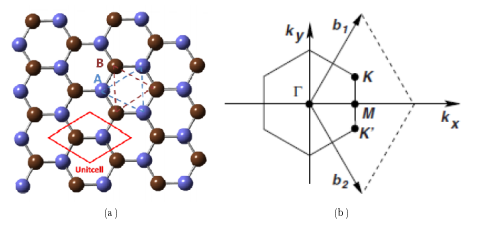
\includegraphics[width=0.7\linewidth]{../Figures/honeycomb_lattice.png}
  \caption{Image from a web source. In Fig. (a) the unit cell is sketched and the sublattices A and B are shown in blue and red respectively. In Fig. (b) the reciprocal lattice is shown, toghether with the high symmetry points $K$, $M$ and $K'$.} 
\label{Fig2.2}
\end{figure}

